\chapter[La biologie structurale au sein d'environnements immersifs et interactifs]{Contexte et état de l'art}
\minitoc
\cleardoublepage


\section{Liste des figures}

\begin{itemize}
	\item Transcription/traduction schématisées
	\item Tableau correspondance triplet ARN -> AA
	\item Cristallographie à différentes résolutions
	\item Champs de force et différence de précision
\end{itemize}

\section{La biologie structurale et l'outil informatique}

L'étude des différents métabolismes régulant la vie des cellules, unité de base constituant l'ensemble des organismes vivants, peut être divisée en plusieurs sous-domaines caractérisés par l'échelle à laquelle les phénomènes sont observés, par la nature des organismes étudiés et par les méthodes utilisés pour les étudier. Parmi ces sous-domaines, la biologie moléculaire s'intéresse à l'étude de la structure et des interactions entre biomolécules (ADN, ARN et protéines) et leur synthèse au sein de la cellule. Elle a pour but d'expliquer des phénomènes biologiques de grandes échelles d'un point de vue moléculaire. La biologie moléculaire se rapproche beaucoup de la biochimie à qui elle emprunte plusieurs techniques et idées. La biochimie s'intéresse à l'étude des phénomènes chimiques régissant les interactions entre les biomolécules. Autre discipline gravitant autour de l'étude des interactions, fonctions et structures des molécules, la biophysique possède une approche plus quantitative de la question et cherche à expliquer les phénomènes moléculaires grâce aux lois physiques régissant le reste du monde. A l'intersection de ces trois domaines d'études se trouve la biologie structurale, domaine spécifiquement intéressé aux structures mêmes des biomolécules, aux étapes permettant à une biomolécule d'acquérir une structure fonctionnelle et aux effets de la structure sur la fonction des biomolécules. C'est un domaine d'étude utilisant plusieurs techniques expérimentales et computationnelles, principalement basées sur des lois physiques, afin d'obtenir une description de précision atomique de la structure des molécules étudiées et de leur dynamique structurelle dans leur environnement cellulaire, impliquant donc les interactions qu'elles peuvent avoir avec d'autres biomolécules et la conséquence sur leur structure, et donc leur fonction.
Il est possible de distinguer plusieurs familles de biomolécules: Les protéines, les acides nucléiques, les lipides, l'eau, etc.. Elles ont en commun leur participation aux processus métaboliques de la cellule, indépendamment ou par des interactions plus ou moins complexes entre-elles. Notre étude porte majoritairement sur les biomolécules naturelles de grandes tailles, appelées également macromolécules, regroupant exclusivement les acides nucléiques et les protéines. Nous aurons une attention particulière sur les protéines même si la portée de nos recherches peut majoritairement s'étendre aux acides nucléiques.

\subsection{Les protéines, unités fonctionnelles du vivant}

Les protéines sont le dernier composant du processus biologique cellulaire le plus important chez les êtres vivants: La transformation de l'information génétique contenu dans l'ADN en unités biologiques fonctionnelles, les protéines. Ce processus passe par deux étapes principales, la transcription et la traduction. La transcription permet de transférer les informations contenues dans le noyau et portées par l'ADN vers le lieu de la traduction, en dehors du noyau cellulaire. Ce transfert se fait grâce à l'ARN, un acide nucléique simple brin, qui est capable de traverser la paroi cellulaire au contraire de l'ADN, double brin sous forme d'hélice et donc structurellement trop gros pour traverser cette paroi. Lorsque les ARN parviennent aux organites cellulaires responsables de la traduction, les ribosomes, elles s'y lient et l'étape de traduction peut commencer. La traduction consiste à transformer l'information génétique de l'ADN, copiée par les ARN, pour former les protéines. Ces deux étapes indispensables à la formation des protéines sont illustrées dans la figure X.

\subsubsection{Genèse}

L'ADN est découpé en séquences codantes et non codantes, les séquences codantes étant responsables de la formation de protéines dans la majorité des cas, alors que les séquences non codantes ne mènent à aucune structure moléculaire. Chaque séquence codante est une suite précise de nuclétotides. Ces nucléoties, au nombre de quatre (Adénine, Thymine, Guanine et Cytosine), constituent la structure de l'ADN. La séquence codante est indispensable aux ribosomes pour générer la protéine que la séquence code. L'ARN intervient donc en se liant à l'ADN et en se structurant de façon à rapporter cette séquence. L'ARN est également composé d'une suite de nucléotides (Adénine, Uracile, Guanine et Cytosine) et se forme par complémentarité au brin d'ADN codant qu'elle lie. Lorsque l'ARN a traversé la paroi cellulaire et s'est liée aux ribosomes, chaque triplet de nucléotides qui la compose est intégrée dans un compartiment du ribosome qui va les mettre en interface avec un groupement moléculaire précis, le composant de base des protéines, les acides-aminés. 
Au sein des protéines présents chez les êtres vivants, 22 acides aminés différents ont été identifiés. Parmi ces 22 acides aminés, 19 d'entre-eux ne sont constitués que de quatre atomes distincts: le carbone, l'hydrogène, l'oxygène et l'azote. Deux autres possèdent également un atome de soufre et enfin le dernier, plus rare, possède un atome de sélénium. Ces acides-aminés possèdent une partie commune qui constitue, lorsqu'ils sont liés, le squelette de la protéine. Ils se différencient par une partie possédant 22 combinaisons et appelée la chaîne latérale. Puisque les nucléotides sont au nombre de 4, il existe 64 combinaisons possibles. Chaque combinaison code, ou est complémentaire, d'un acide-aminé particulier. En moyenne, un acide-aminé est codé par 3 combinaisons de triplets de nucléotides différents comme illustré dans la figure X. Chaque triplet de nucléotide de la séquence ARN est donc associé à un acide-aminé. Tout au long du passage de l'ARN dans le ribosome, la protéine est formée séquentiellement, par complémentarité aux différents triplets. Quand le triplet de nucléotide codant pour l'arrêt de la traduction, la protéine est détachée du ribosome et va évoluer au sein de la cellule vers son lieu d'action.

\subsubsection{Structure} 

Une protéine est donc constituée d'une succession d'acides-aminés. La chaîne latérale de ces acides-aminés, de part sa structure moléculaire différente entre les 22 acides-aminés, donne lieu a des propriétés physico-chimiques différentes. Il est possible de classer ces acides-aminés selon plusieurs critères, depuis leur taille jusque leur propriété hydrophobique (affinité avec l'eau) ou leur polarité. Il existe cependant un classement commun qui les regroupe en six groupes fonctionnels: Les acides-aminés aliphatiques (Glycine, Alanine, Valine, Leucine et Isoleucine), les acides-aminés avec groupement hydroxyle, sulfurique ou sélénique (Sérine, Thréonine, Méthionine, Cystéine et Sélénocystéine), les acides-aminés cycliques (Proline), les acides-aminés aromatiques (Phénylalanine, Tyrosine et Tryptophane), les acides-aminés basiques (Histidine, Lysine et Arginine) et enfin les acides-aminés acides et leurs amides (Aspartate, Glutamate, Asparagine et Glutamine).
La séquence des acides-aminés est appelée la structure primaire d'une protéine. Les propriétés physico-chimiques des différents acides-aminés entrainent la mise en place de motifs particuliers. Ces motifs structuraux sont au nombre de 3, hélices, feuillets et boucles même si chaque motif possède cependant quelques variations structurelles légères. L'enchainement de ces motifs d'acides-aminés est appelée la structure secondaire. 
Enfin, les protéines possèdent également des motifs plus importants, souvent le résultat de l'agencement particuliers des motifs de structures secondaires cités précédemment. Parmi ces motifs, on peut citer les structures ????
C'est l'ensemble de ces différents niveaux de structuration qui forme la structure tertiare et 3d de la protéine.
Cette structuration, appelée aussi repliement de la protéine, se déroule pour sa majorité après l'étape de traduction effectuée par le ribosome. Le repliement s'effectue grâce à des molécules particulières, appelées molécules chaperonnes, qui viennent se lier à la protéine pour lui faire adopter sa structure 3d dites stable. La majorité des protéines ne peuvent pas être fonctionelles sans structuration stable car leur action provient de liaisons avec des molécules partenaires dont certains atomes vont reconnaitre des acides-aminés précis de la protéine. Si ces acides-aminés venaient à être rendus inaccessibles à cause d'une mauvaise structuration ou si l'ensemble des acides-aminés impliqués dans la liaison avec la molécule partenaire ne se trouvaient pas dans le même voisinage géométrique alors la liaison serait impossible et donc l'action de la protéine ne pourrait se faire. C'est la raison pour laquelle la biologie structurale accorde une importance primordiale à la structure, brique de base de la fonction des protéines.


\subsubsection{Techniques expérimentales}

Les techniques expérimentales utilisées en biologie structurale pour obtenir la structure tertiaire de biomolécules sont relativement coûteuses de part leur complexité. En effet, les techniques de microscopie optique standards ne peuvent permettre aujourd'hui une observation à l'échelle atomique, quel que soit l'objet d'étude. Ce sont donc des méthodes physiques indirectes qui sont principalement utilisées afin d'obtenir des informations sur la structure 3d d'une biomolécule à l'échelle atomique. La plupart de ces techniques mettent en jeu des instruments de mesure de haute technologie et parfois une préparation complexe de l'échantillon nécessitant un effort scientifique important.

\paragraph{Cristallographie à rayons X ou radiocristallographie}

Parmi ces techniques expérimentales, la plus ancienne et la plus utilisée, principalement pour sa précision, est la cristallographie aux rayons X ou radiocristallographie. Cette technique consiste à envoyer un faisceau de rayons X sur un cristal composé exclusivement de la biomolécule étudiée. La mesure des angles et de l'intensité des rayons réfractés permet d'obtenir une image tridimensionnelle de la densité électronique dans le cristal. A partir de cette densité, il est possible d'obtenir la position moyenne des atomes présents dans le cristal ainsi que les liens existants entre-eux en superposant la séquence d'atomes, connue, dans la carte de densité électronique ainsi obtenue. 
L'avantage de la radiocristallographie est sa très grande précision et l'absence de limite de taille pour le cristal, permettant l'observation de structures moléculaires de très grande taille comme les ribosomes (environ un million d'atomes). Suivant les biomolécules observées, il est possible d'obtenir des structures tridimensionnelles à des résolutions comprises entre 2 et 3\r{A} (Angströms = \SI{e-10}{\metre}) pour une précision sur la position des atomes autour de 0.5\r{A}. 1\r{A} de résolution permet une précision atomique quasi-parfaite. Les cartes de densité et les modèles atomiques créés à partir de ces cartes sont illustrés dans la figure X. 
Certaines biomolécules sont néanmoins très difficiles à cristalliser et on évalue à environ un quart la proportion de macromolécules permettant de créer un cristal de taille et de qualité suffisante de diffracter suffisamment les rayons X. Cette cristallisation est une étape peu facilement automatisable et qui se révèle majoritairement empirique, demandant un travail spécifique en plus de l'application de la technique. Les hydrogènes présents dans les macromolécules sont très difficiles à percevoir du fait de leur très faible densité électronique. L'obtention d'une structure 3d par radiocristallographie est relativement fastidieuse et nécessite en moyenne plusieurs mois de travail.

\paragraph{Spectroscopie à Résonance Magnétique Nucléaire (RMN)}

Également très utilisée, la RMN consiste à envoyer une séquence précise d'impulsions électromagnétiques sur une molécule en présence d'un champ magnétique. La fréquence et la séquence des impulsions électromagnétiques sont propres à chaque type d'atome. Cette technique se base sur les mouvements de rotation naturels des atomes, créant un mini champ magnétique (ou spin). Seuls quelques atomes sont adaptés à la spectroscopie RMN car ils possèdent un spin nucléaire de 1/2. En biologie structurale, c'est principalement le proton H\textsuperscript{1} qui est ciblé. Les noyaux atomiques possédant des spins sont excités par les impulsions électromagnétiques et absorbent l'énergie ainsi reçue. Lors de l'étape de relaxation suivant l'impulsion, les noyaux atomiques relâchent de l'énergie sous forme de résonance à différentes longueurs d'onde, calculée et reportée par les instruments de mesure. Cette résonance varie en fonction de la nature de l'atome excité et de son environnement. Il est donc possible, grâce à ces résonances, pour un atome donné, d'avoir des informations sur la nature et le nombre d'atomes voisins, la liaison chimique dans laquelle il est impliqué, sa distance à d'autres atomes, sa mobilité, etc... A la différence de la cristallographie, la RMN peut s'appliquer sur une solution composée de la molécule étudiée et il est de fait plus aisé de stabiliser une molécule en solution que de la cristalliser. Il est également possible d'avoir des informations sur la dynamique de la molécule puisqu'au contraire de quand elle se trouve dans un cristal, une molécule en solution n'est pas statique.
L'état dynamique de la molécule est aussi un inconvénient pour obtenir une structure 3d fixe puisque la précision de la mesure sera perturbée par les changements structurels de la molécules. L'un des autres inconvénients de la spectroscopie RMN est la taille des molécules observée du fait de la complexité du traitement des signaux de résonance magnétique, ces derniers se superposant sur un spectre de largeur fixe. Ainsi, plus le nombre d'atome est important, plus le nombre de signaux augmentera et s'accumulera sur un spectre de largeur constante. La taille optimale pour la RMN varie entre 10 et 50 kilo-Dalton (kDa) correspondant à des molécules de 1.500 à 10.000 atomes. de plus, Pour les plus grosses molécules, il est nécessaire d'effectuer un marquage isotopique permettant d'obtenir un spectre non plus 2d mais 3d où les atomes ciblés, en plus de H\textsuperscript{1}, sont le C\textsuperscript{13} et le N\textsuperscript{15} après enrichissement spécifique de la biomolécule observée.

\paragraph{Cryo-microscopie électronique}

Autre technique populaire en biologie structurale, la cryo-microscopie électronique consiste à utiliser le principe de la microscopie électronique, et donc d'utiliser un faisceau de particules d'électrons au lieu de rayonnements électromagnétiques comme en microscopie optique, sur un échantillon préalablement cryogéniser lors de l'étape de fixation. Le faisceau de particule d'électrons passe au travers de lentilles électrostatiques et électromagnétiques puis au travers de l'échantillon où il est modifié pour former une image électronique finalement amplifiée par d'autres lentilles et projetée sur un scintillateur. 
La particularité de la cryofixation de l'échantillon, par opposé à la fixation chimique ou la déshydratation, est que l'échantillon est amené très rapidement à la température de l'azote liquide (\SI{-195.79}{\degreeCelsius}) ou de l'hélium liquide (\SI{-269}{\degreeCelsius}) afin que la glace formée ne soit pas cristalline et que le spécimen étudié conserve son état naturel. Pour des biomolécules, cela assure une conservation d'une structure 3d stable de la molécule. La cryo-EM permet d'étudier des structures moléculaires de grandes tailles, à partir de 300kDa jusqu'à des tissus de plusieurs centaines de nanomètres, en passant par les ribosomes, les virus ou les composants cellulaires.
Bien qu'en constante développement, la cryo-EM possède une résolution relativement faible comparée aux deux techniques précédentes puisque les cartes de densité obtenues par cette technique ne permettent pas une résolution de moins de 4\r{A} pour les cartes les plus précises\cite{zhou_atomic_2011}. L'exposition de l'échantillon à un faisceau de particules d'électrons, combiné à sa cryogénisation, dommage significativement l'échantillon qui ne peut être réutilisé ensuite.

\paragraph{Diffusion des rayons X - SAXS}

La technique SAXS est basée sur les interactions élastiques entre les photons et les nuages électroniques. Cette technique s'inspire directement de la diffraction des rayons X quand ils traversent un cristal (diffraction de Bragg) entraînant la diffusion de ces rayons à différents angles de l'ordre de la dizaine de degrés. L'angle de diffraction est inversement proportionnel à la distance interatomique des atomes présents dans le cristal. Or, les informations nécessaires pour constituer la structure 3d de macromolécules concernent des distances trop grandes pour que les angles de diffraction soient facilement détectables. Il est nécessaire d'utiliser un rayonnement X monochromatique très proche de l'échantillon constitué de la biomolécule d'intérêt.De la même manière que pour les précédentes techniques, une carte de densité, ici densité électronique, est ainsi générée après interprétation des angles de diffraction calculés par l'instrument de mesure placé à la suite du faisceau émis à travers l'échantillon.
L'un des avantages de la technique SAXS par rapport à la cristallographie est l'absence de cristal pour effectuer l'expérience, l'échantillon étant mis en solution. Mais cet avantage est terni par la résolution de la technique qui ne permet pas d'avoir une description atomique d'une biomolécule. Elle est souvent utilisée pour obtenir une structure 3d approximative de complexes moléculaires ou de composants cellulaires de grandes tailles. Une de ces forces repose aussi sur la rapidité de l'expérience qui, en combinant l'ensemble des étapes de préparation, expérimentation et analyses des résultats, peut générer une carte de densité en quelques jours.

\subsubsection{Approches bio-informatiques}


En complément de ces analyses expérimentales, il est possible, et commun, d'utiliser des approches computationnelles afin de compléter les informations structurelles recherchées. Ces approches dites \textit{in silico} sont moins coûteuses que les approches expérimentales mais souffrent d'une précision moindre et surtout d'un facteur de confiance significativement moins important que les approches énoncés précédemment. Les approches computationnelles ont cependant beaucoup évoluer ces deux dernières décennies, portées par l'essor de l'informatique. La puissance de calcul des outils informatiques permettent désormais d'intégrer des paramètres physico-chimiques à toute simulation numérique cherchant à créer des modèles 3d cohérents de biomolécules à partir de leur simple séquence primaire. Le fossé préalablement existant entre la précision des techniques expérimentales et computationnelles diminue donc rapidement même si pour le moment les résultats obtenus par méthodes computationnelles sont dans la grande majorité des cas vérifiés expérimentalement. Ces approches font parti d'un vaste domaine appelé bio-informatique et qui regroupe l'ensemble des outils informatiques permettant de répondre à des problématiques biologiques. En bio-informatique structurale, les outils bio-informatiques traitent de la reconstruction, de la prédiction ou de l'analyse de la structure 3d et/ou du repliement des biomolécules, protéines ou acides nucléiques. Ils peuvent être regroupés en plusieurs catégories suivant leur place dans le processus d'obtention d'informations structurelles, leur intégration plus ou moins importante au sein des techniques expérimentales et les algorithmes qu'ils mettent en jeu. On peut donc distinguer: Les systèmes de bases de données, les programmes de modélisation moléculaire et les programmes de visualisation scientifique.

\paragraph{Prédiction de structure moléculaire}

La prédiction de structure 3d moléculaire \textit{in silico} est la capacité de générer des modèles de structures 3d de biomolécules à partir d'un ensemble restreint de données. Ces données peuvent être simplement la structure primaire d'une protéine, on parle alors de prédiction \textit{ab initio}, ou bien provenir de résultats expérimentaux et/ou computationnels, on parle alors de prédiction guidée. Ces deux approches ont en commun les algorithmes scientifiques qu'elles utilisent afin de générer les modèles 3d de protéines et regrouper dans une approche: la dynamique moléculaire. La dynamique moléculaire cherche à modéliser l'évolution d'un système de particules au cours du temps en simulant des conditions de température, pression, etc... identiques aux conditions cellulaires afin d'observer l'évolution d'une système biologique précis.

Une dynamique se base en premier lieu sur la mise en place d'une structure 3d de départ. Cette structure de départ est plus ou moins proche de la structure 3d finale suivant la quantité et la précision des données utilisées en entrée. Dans l'approche \textit{ab initio} où aucune information est utilisée en entrée, la structure de départ n'est que la séquence primaire de la protéine, à savoir un enchaînement d'acides-aminés. 
Dans une seconde étape de préparation de la simulation numérique, la structure de départ est introduite dans un environnement atomique, modélisé informatiquement, cherchant à refléter le plus fidèlement possible l'environnement cellulaire dans lequel la protéine évolue \textit{in vivo}. Cet environnement peut être représenté simplement au moyen d'une boîte contenant des molécules d'eau où la protéine sera plongée, ceci constitue un des environnements les plus basiques et les plus utilisés. Dans des environnements plus complexes il est possible de retrouver les ions présents habituellement autour de la protéine ou des structures complexes représentant une partie de composant cellulaire au sein duquel évolue habituellement le complexe moléculaire étudié telle que la membrane cellulaire. 
La complexité de l'environnement n'est pas seulement dépendant de sa composition et de la richesse de sa représentation mais également du degré de précision choisi pour le modéliser. Nous détaillons les différents degrés de précision d'une modélisation moléculaire ci-après.

Lorsque la structure de départ et l'environnement ont été défini la simulation moléculaire peut débuter. Une simulation moléculaire commence par donner une énergie de départ au système moléculaire (protéine + environnement) afin de le mettre en mouvement. Chaque déplacement de particules pendant la simulation est régit par des équations mathématiques correspondant aux lois physiques connus s'appliquant habituellement dans une cellule. Ces équations comportent comme paramètres: Les conditions physiques de l'environnement (température, pression, etc..) et les propriétés physiques des particules (polarité, charge, taille, etc...). Ces paramètres sont renseignés au sein d'un champ de force décrivant l'énergie potentiel d'un système. Plusieurs champs de force sont utilisés lors de simulations numériques et le choix d'un champ de force dépend essentiellement de l'environnement dans lequel est modélisé le complexe moléculaire d'intérêt ainsi que le degré de précision utilisé pour décrire les particules du système (tout-atome, atomes unifiés, gros grains, etc...). Ce degré de précision influe sur l'exactitude des paramètres utilisés dans les équations mathématiques. Les champs de force tout-atome considèrent par exemple tous les atomes du système moléculaire simulé indépendamment. Ceci implique un nombre important de calculs et donc un temps de simulation important. Afin de réduire le nombre de calculs il est donc possible de réduire la précision et donc d'ignorer certains atomes dont l'impact sur la simulation est négligeable, tels les hydrogènes. Il est également possible de considérer certains groupes d'atomes particuliers comme une seule particule dont les paramètres physico-chimiques sont le résultat d'une moyenne des atomes qui la composent. Différents champs de force sont illustrés dans la figure X.

Les paramètres physiques comme la température, la pression ou les forces d'attraction et de répulsion atomiques sont appliquées et permettront au système d'évoluer vers différents niveaux énergétiques. L'énergie potentielle d'une structure est directement liée aux positions des particules du système et sa valeur reflète les énergies mises en jeu dans les interactions inter-atomiques du système. Dans une simulation moléculaire, on cherche à faire parcourir à la structure étudiée son paysage énergétique afin de trouver le minimum énergétique global, et donc le plus stable pour cette structure. Cet état de stabilité doit normalement refléter l'état de la protéine étudiée dans son environnement naturel cellulaire. La complexité de la surface énergétique d'une molécule est proportionnel à la complexité même de la molécule, principalement sa taille. Il est rare de trouver le minimum global d'un paysage énergétique au cours d'une simulation, on cherche donc dans la majorité du temps des minimums locaux les plus bas possibles. Tout au long de la simulation, les coordonnées 3d de la structure sont sauvegardées afin de pouvoir rejouer la trajectoire de la simulation à tout moment au moyens de programmes de visualisation 3d. Chaque pas de la simulation correspond à un set de coordonnées 3d qui est associé à une valeur d'énergie potentielle permettant de savoir quelle configuration géométrique correspond aux énergies potentielles de la protéine les plus bas.

\paragraph{Analyses et interprétation de simulations}

Les simulations numériques génèrent, en plus des coordonnées 3d du complexe moléculaire au cours du temps, plusieurs informations importantes pour l'interprétation des évolution structurelles. Ces informations sont pour la plupart des valeurs énergétiques associées à chaque pas de la simulation. Dans le but de préciser la description du système, d'autres valeurs peuvent être générées à partir de ces informations. Cet ensemble de données propres à la simulation doivent permettre de comprendre les phénomènes se déroulant au cours d'une simulation. Il est donc crucial d'interpréter ces informations et de les lier aux états structurels de la molécule et d'ainsi comprendre exactement les mécanismes impliqués dans les changements structuraux observés. Les analyses post-simulation permettant d'extraire des informations de la trajectoire sont souvent intégrées dans la suite d'outils ayant été utilisée pour la simulation (AMBER \cite{pearlman1995amber}, CHARMM \cite{brooks2009charmm}, GROMACS \cite{pronk2013gromacs} pour les plus connus d'entre-eux). Cependant, plusieurs bibliothèques ont également été conçues afin de permettre d'utiliser certains algorithmes et outils d'analyses de simulation moléculaire en dehors des suites logicielles dédiées (BioPython \cite{cock_biopython:_2009}, MDAnalysis \cite{michaud-agrawal_mdanalysis:_2011}, MDTraj \cite{McGibbon2014MDTraj} par exemple). 

\paragraph{Systèmes de bases de données moléculaires}

Les SGBD permettent de regrouper l'ensemble des informations scientifiques obtenues au cours de l'histoire et les mettre à disposition de la communauté scientifique. Ceci peut se faire grâce à leur intégration au sien de portails biologiques gérant la conformité des données aux standards du domaine, leur accès à l'ensemble des scientifiques et éventuellement leur association avec des données d'autres domaines scientifiques proches.

L'une des bases de données les plus utilisée en biologie structurale est la \textit{Protein Data Bank} \cite{berman_protein_2000} qui regroupe l'ensemble des structures 3d de protéines publiées et vérifiées dans plusieurs formats standards et acceptés par la majorité des outils bio-informatiques structuraux. Les structures 3d présentes dans la PDB proviennent de techniques diverses (POURCENTAGE PAR TECHNIQUE).

Parmi les informations stockées dans des bases de données et utilisées en biologie structurale on retrouve: les profils biologiques des protéines avec leur structure primaire/secondaire/tertiaire, leur environnement cellulaire, leur rôle, etc... (SWISSPROT+TrEMBL \cite{boeckmann2003swiss}, PDB,...); les réseaux d'interactions moléculaires (interactome) mettant en avant les partenaires moléculaires déjà identifiés (STRING \cite{Snel15092000}, CCSB Interactome Database \url{http://interactome.dfci.harvard.edu/},...); les évolutions génomiques des séquences d'ADN codantes identifiant les régions évoluant rapidement au sein des protéines (séquence primaire changeante) et les régions plus stables et donc potentiellement importantes pour la fonction métabolique de la protéine (USCS \cite{kent2002human}, Ensembl \cite{hubbard2002ensembl},...). 

Certaines de ces bases de données sont mises en relation au travers de portails biologiques permettant de regrouper toutes les informations sur une protéine au sein d'un même espace.

\paragraph{Visualisation moléculaire 3d}

Les programmes de visualisation moléculaire 3d permettent d'observer, dans un espace graphique 3d, des molécules, à partir de fichiers de coordonnées 3d. Ces logiciels permettent principalement de mettre en avant certaines des particularités structurelles des molécules observées via des jeux de couleurs ou de formes particuliers et largement adoptés dans la communauté. Ces programmes s'appuient sur différents formats de fichier pour ces coordonnées même si la plupart sont capables de lire au moins le format PDB. Au-delà de la visualisation statique de structures 3d, il est souvent possible d'utiliser ces programmes afin de lire la trajectoire d'une simulation numérique. Ainsi, il est possible d'observer l'évolution structurelle d'un complexe moléculaire au cours du temps ou d'observer des phénomènes biologiques se déroulant au cours du temps (passage de molécules au travers d'une membrane, repliement d'une région protéique suite à son interaction avec un partenaire biologique, etc...). Parmi les programmes de visualisation 3d largement utilisés aujourd'hui nous pouvons citer: 
\begin{itemize}
	\item \textbf{PyMol} \cite{delano_pymol_2002}, basé sur le langage Python et offrant une API pour ce langage, il dispose de nombreux rendus visuels et est, selon l'auteur original, utilisé dans plus d'un quart des images de structures moléculaires présentes dans les articles scientifiques.
	\item \textbf{VMD} \cite{humphrey_vmd}, spécialisé dans la visualisation et l'analyse de résultats de simulations de dynamiques moléculaires, cet outil est très usité du fait de ses nombreuses extensions et la possibilité de le relier à NAMD, un programme de dynamique moléculaire, permettant ainsi d'effectuer des simulations moléculaires interactives.
	\item \textbf{Jmol} \cite{herraez2006biomolecules}, basé sur Java et disponible sous forme d'application indépendante ou intégrée dans des pages web, ce visualiseur est populaire du fait de sa facile intégration au sein de contenus web. Il offre de plus plusieurs rendus graphiques très performants.
\end{itemize}

Cette liste est non-exhaustive mais recense trois des logiciels de visualisation moléculaire les plus utilisés dans le monde scientifique et plus particulièrement en biologie structurale.

Les programmes de visualisation 3d sont aujourd'hui disponibles sur de nombreux supports. En plus de leur présence pour une utilisation sur des moniteurs 2d habituels, il est possible de les utiliser sur des plateformes mobiles (smartphones/tablettes) ou dans des environnements immersifs 3d (visiocasques/systèmes CAVE).

\section{Réalité virtuelle et interactivité}

La contribution de la Réalité Virtuelle (RV) dans le monde scientifique est relativement récent mais connaît un essor très important depuis quelques années. Cet essor peut être expliquer par deux raisons principales: La démocratisation des dispositifs de réalité virtuelle et augmentée et l'apport de la 3d pour observer des données complexes et/ou intrinsèquement 3d. Comme nous l'avons souligné auparavant, la génération de données est arrivée aujourd'hui à une vitesse haut-débit et dépasse depuis longtemps les capacités d'interprétation de résultats disponibles. Il est donc crucial de trouver un moyen de rapprocher les processus d'analyses des processus de génération de données. Il n'est aujourd'hui pas pensable de réduire la quantité de données générée, il convient donc de mettre en place des solutions d'analyses adaptées, à la fois efficaces et précises et se rapprochant le plus possible des générateurs de données afin d'y filtrer le surplus inutile. La RV, grâce à sa capacité à créer un monde artificiel où les informations peuvent être mêlées entre-elles tout en gardant leur signification est toute adaptée pour répondre au défi de l'optimisation des processus d'analyses. 

\subsection{Définition}

Plusieurs définitions de la RV ont été proposé depuis son émergence dans les années 90. Sherman et Craig définissent la RV comme le fait d'être immergé dans un monde virtuel interactif \cite{sherman2002understanding}. Brooks formule cette définition de manière presque similaire en disant que la RV est une expérience où l'utilisateur est efficacement immergé dans un monde virtuel réactif \cite{brooks1999s}. De façon légèrement différente, Burdea décrit la RV comme une simulation dans laquelle les graphismes générés par informatique sont utilisé pour créer un monde au rendu réaliste qui n'est pas statique mais répond aux sollicitations de l'utilisateur \cite{burdea2003virtual}. On retrouve dans ces définitions les trois piliers qui définissent la RV selon Heim : Immersion, Interaction, Information \cite{heim1998virtual}. Bien qu'il soit difficile d'extraire une définition simple et unique de la RV, l'idée principale est bien de mettre l'utilisateur au centre d'un environnement créé artificiellement mais assez proche de la réalité pour lui permettre d'y évoluer de la façon la plus naturelle possible. Cette immersion de l'utilisateur passe par la mise en place de retours sensoriels précis et réalistes qui vont amener l'utilisateur à considérer le monde virtuel comme un monde plausible. L'interaction est donc primordiale puisqu'un utilisateur va attendre de la part du monde dans lequel il évolue un retour d'information suite à ses actions. Ces retours d'informations peuvent être de différentes formes, souvent visuels, ils peuvent en fait s'adresser à l'ensemble des sens de l'utilisateur. C'est la richesse de ces retours qui définira le degré d'immersion de l'utilisateur et donc son implication dans le monde virtuel. Bowman et McMahan notent qu'il n'est cependant pas nécessaire de gérer l'ensemble des sollicitations sensorielles d'un utilisateur pour assurer une immersion acceptable \cite{bowman_virtual_2007}. Dans cette même étude, les auteurs proposent un découpage de l'immersion en plusieurs composants, invoquant une immersion qui n'est jamais soit absente, soit parfaite. Ils vont même plus loin en évoquant les applications de RV où la présence de l'utilisateur n'est pas primordiale. Dans ces applications, la perception du monde virtuel et de son contenu passe avant la sensation de présence de l'utilisateur. Parmi ces applications, la visualisation de données scientifiques, qui nous intéresse dans notre étude, met davantage l'accent sur le contenu que sur l'effort pour immerger l'utilisateur dans un monde virtuel. 

\subsection{La réalité virtuelle pour les données scientifiques}

La RV possède plusieurs facettes répondant naturellement aux problèmes posés par l'analyse scientifique. Rappelons la problématique actuelle de la visualisation de données scientifiques. Les données générées excèdent de loin les capacité d'interprétation disponibles. De plus, la complexité et la quantité des données est telle que leur rendu 2d ou 3d sur des écrans d'ordinateur ne sont plus suffisants pour rapporter l'ensemble des informations que les données contiennent. L'accès à certaines informations est donc entravée et enfouie sous la quantité de données à analyser par l'utilisateur. 
Dans le cadre de la visualisation scientifique, on peut considérer que la capacité d'affichage stéréoscopique doublé à une surface d'affichage à 360 degrés est la facette la plus importante de la RV. Plusieurs études ont par exemple démontré que la perception de la profondeur lors de la représentation de structures moléculaires apportait une aide non négligeable pour leur compréhension structurelle \cite{van_dam_immersive_2000,stone_immersive_2010}. Les complexes moléculaires et les protéines sont par nature structurées en 3d et c'est cette structuration qui est au coeur des études en biologie structurale. La stéréoscopie est donc une alternative naturelle pour l'observation de structures protéiques puisqu'elle utilise la compréhension innée de la 3d du cerveau humain pour analyser des phénomènes et objets de nature 3d. 
Mais l'étude de la structure seule ne peut suffire lors de l'étude d'un complexe moléculaire, nous avons souligné auparavant la présence de nombreuses données accompagnant la génération de modèles 3d lors d'une simulation moléculaire. Ces données, sous forme de valeurs brutes, doivent être également analysées. La dimension de profondeur propre à la stéréoscopie prend une nouvelle fois tout son sens ici. Ce n'est plus la nature 3d même des données observées qui va rendre cette profondeur importante, puisque nous nous intéressons maintenant à des valeurs numériques brutes, mais la possibilité d'utiliser une 3e dimension pour représenter des modèles, des tendances ou bien des anomalies au sein des données affichées.
Au delà de la stéréoscopie, la surface, ou davantage le volume quand on parle de 3d, disponible dans les dispositifs de RV pour afficher des informations est beaucoup plus important que ce qu'on peut retrouver au sein de dispositifs 2d standards. Combiné avec un suivi de l'orientation et de la position de la tête de l'utilisateur, il devient aisé de créer un monde composé de 360 degrés d'informations accessibles simplement et rapidement au moyen d'un simple mouvement de tête ou coup d'oeil.

Un autre apport de la RV que l'on peut citer se trouve dans les techniques d'interaction qu'elle met en jeu et favorise. Les interactions directes, regroupant les interactions mettant en jeu des mouvements et gestes de l'utilisateur pour interagir avec son environnement virtuel, font opposition aux interactions indirectes comme peut l'être le clavier ou la souris. Ces interactions directes sont souvent beaucoup plus intuitives et implique une certaine proximité de l'utilisateur avec les données puisque ce sera principalement son corps qui déclenchera l’événement d'interaction. Cependant, il est bon de noter que ces interactions ont souvent une courbe d'apprentissage plus longue que les interactions indirectes. De plus, elle demande souvent une précision plus importante et sont donc soumises à des variations d'efficacité parfois plus importantes. La notion d'interaction n'intervient pas que dans un sens unique et même si la méthode permettant d'interagir avec un objet est primordiale, le retour sensoriel provoqué par l'interaction est, en RV, un sujet d'étude à part entière. Nous avons vu que ces retours sensoriels participent à l'immersion ressentie par l'utilisateur dans un monde virtuel mais ils peuvent également servir de repères ou de vecteurs d'informations importants. Même s'il est possible de mettre en place certaines sollicitations autres que visuelles lors d'un travail sur un poste de travail standard, il est très rare de trouver des retours sonores ou haptiques lors d'une session de travail. Au delà de la limite potentielle matérielle, un retour haptique impliquant par exemple la nécessité de posséder un dispositif muni d'un système de retour d'effort, les limites sont souvent logicielles, peu de programmes implémentent des retours sensoriels autres que visuels dans le design de leurs outils d'analyses de données. Il est au contraire très commun de prendre en compte ces retours sensoriels lors du développement de solutions logicielles dédiées à la RV. La RV est par essence définie par l'implication de l'utilisateur. Il a donc dû développer très tôt des moyens pour retranscrire un maximum de sensations aux utilisateurs lors de leurs expériences virtuelles. En visualisation de données abstraites et/ou scientifiques, l'utilisation de ces méthodes de retours sensoriels a pu ensuite être détourné de leur but premier, l'immersion, pour communiquer des informations supplémentaires à l'utilisateur pendant ses phases d'interactions. La possibilité par exemple de déclencher un événement sonore lors de la sélection de données critiques ou extrêmes dans un set de données est l'un des exemples de l'utilisation d'un retour auditif pour transmettre une information.



\subsection{Paradigmes d'interaction en immersion}

\section{Visualisation analytique}

\subsection{Visualisation analytique interactive pour les données scientifiques}

\subsection{Représentation des connaissances}

\subsubsection{Bio-ontologies}

\cite{schulze-kremer_ontologies_2002}

\subsubsection{Web sémantique et formalismes à base de graphes}

Sesame [55] est une architecture générique pour le stockage persistant de RDF(S) dans une base de données et l'interrogation de ce RDF(S) avec le langage RQL. RQL [56] est un langage de requête RDF défini par le moyen d'un ensemble de requêtes fondamentales, un ensemble de filtres de base et un moyen de construire de nouvelles requêtes par une composition fonctionnelle et des itérateurs. Lors de l'analyse d’une requête RQL, Sesame construit une requête optimisée évaluée au moyen d'une série d'appels à la couche de stockage et d’inférence de Sesame.

Par comparaison RDQL [56] permet l'interrogation de données RDF au niveau de la structure, tandis que Sesame permet l’interrogation au niveau sémantique. En ce sens notre objectif est beaucoup plus proche de Sesame. Toutefois Sesame ne considère pas la sémantique des XSD datatypes, ni ne permet d’avoir des règles d'inférence exploitant les ontologies.

Jena [57] est l’un des moteurs actuels les plus complets et propose une persistance en mémoire ou en base de données. Il implante RDF, RDFS et OWL ainsi que les requêtes SPARQL et propose un moteur en chaînage avant (RETE), arrière (programmation logique) et hybride. Ce moteur est utilisé pour implanter la sémantique de RDFS et OWL. Le modèle de Jena repose sur une structure prédéfinie de bases de données.

Triple [58] est un langage de requêtes pour divers modèles de données du web sémantique. Le noyau Triple est un langage de requête RDF fondé sur la logique de Horn étendue par des fonctionnalités syntaxiques pour intégrer des primitives RDF comme les espaces de nommage, les ressources et les réifications. Ce langage peut être compilé en logique de Horn et exécuté par des moteurs Prolog. Triple n'est pas limité à l'interrogation de données RDF. Il dispose d'une architecture en couche lui permettant d'interroger d’autres modèles de données avec différents types de sémantique (ex : RDFS et DAML + OIL) et en ce sens il rejoint notre certitude qu’il faut abstraire les structures et algorithmes des différents langages que nous manipulons. Le noyau de Triple est étendu par des règles pour l’axiomatisation de la sémantique de RDFS ; elles peuvent être utilisées avec un moteur d'inférence pour dériver des connaissances supplémentaires à partir d'un schéma RDFS.

DAMLJessKB [59] et son successeur OWLJessKB ainsi que le cœur du eWallet [13] sont des outils de raisonnement pour DAML [60] ou OWL Lite. Ils ont tous les trois intégré JESS [61] un moteur de règles de production qu’ils appliquent à la sémantique de RDF, RDFS, DAML, XSD (XML Schema Datatypes [62]) et OWL Lite. Ils implantent une traduction des triplets RDF vers des faits du langage CLIPS de Jess et utilisent des règles de production pour décrire la sémantique des langages traduits. A l'aide de Jess, ces systèmes peuvent effectuer des raisonnements sur les classes et les instances.

OntoBroker [63] et son successeur On2broker sont des pionniers des systèmes à base d'ontologies basés sur les Frame Logics. OntoBroker gère des métadonnées intégrées dans des documents HTML avec des balises tout comme On2Brocker gère des annotations RDF. Dans les deux systèmes, les ontologies et les requêtes sont exprimées en langage frame logics qui permet la représentation d'une hiérarchie de types de concepts, d'une hiérarchie de types de relations et de règles. Le moteur de requête traduit ces représentations en Logique de Horn pour répondre à une requête.

OntoBroker, On2Broker, DAMLJessKB, OWLJessKB et partagent avec notre initiative le même principe général et les expressivités de leurs langages de représentation à base d’ontologie sont comparables. Toutefois, ces systèmes sont dédiés à des capacités générales de raisonnement sans exploiter les structures de graphes par exemple pour optimiser des opérations spécifiques à la recherche d'informations. Leurs langages de requêtes sont proches des logiques sur lesquelles ils se basent et restent dans leurs limites.

WebKB [64] [65] est un pionnier des serveurs web d'ontologies et des robots web basés sur les graphes conceptuels. Sur la base de sa simplicité et de l'exhaustivité de sa représentation, ses auteurs rejettent l'utilisation directe des langages basés sur XML. WebKB interprète et traduit automatiquement en graphes conceptuels des déclarations exprimées dans une notation linéaire des graphes et intégrées à des documents web. WebKB fournit des commandes de requête pour interroger les propriétés lexicales ou structurelles des documents HTML ou afficher des spécialisations ou généralisations d'un concept, d'une relation ou d'un graphe.

OntoSeek [66] est un autre système conçu pour la recherche d’information basée sur le contenu de pages jaunes et de catalogues de produits en ligne. Il combine les graphes conceptuels et des ontologies du domaine correspondant. Il met l'accent sur les contraintes lexicale et sémantique dans le codage des ressources en graphes conceptuels et la construction de requêtes. Requêtes et annotations des ressources sont des graphes conceptuels lexicaux entre lesquels on cherche des homomorphismes.

WebKB, OntoSeek et la plate-forme que nous spécifierons en section 3.3.4 partagent le même type de représentation à base de graphes, par conséquent, le même principe d’homomorphisme correspondant à une requête sur les graphes d'annotation en prenant en compte la subsomption des types de concepts et des types de relations. Mais ni WebKB ni OntoSeek n’intègre RDF(S) ou les règles dans leur représentation à base d’ontologie.

Avec la standardisation de OWL DL, les moteurs à base de logiques de descriptions ont pris une importance particulière. Citons : Fact et son successeur Fact ++ [67], KAON2 [68] (une branche de KAON qui lui est resté focalisé sur RDFS), Racer [69], Pellet [70]. Ces moteurs offrent des opérations classiques en logiques de descriptions : identification, classification, validation. L’interrogation se limite en général à des requêtes conjonctives et les mécanismes d’interrogation ne sont pas prévus pour exploiter la structure des graphes ni accepter des graphes de grande taille.

En conclusion, aucune des contributions citées ci-dessus ne cherche à mettre en place un modèle pivot et une plate-forme ouverte et open-source pour implanter efficacement les aspects des représentations relevant des graphes. Elles sont toutes liées à un langage particulier (le plus souvent une logique) et/ou à une application particulière.

En ce qui concerne les outils permettant de raisonner avec des graphes conceptuels, les deux principaux outils sont : CoGITaNt [71] développé conjointement par le LIRMM et le LERIA, plate-forme dédiée à la mise en œuvre de mécanismes de raisonnement sur les graphes conceptuels spécifiquement ; et Amine (développé par l'INSEA au Maroc), plate-forme dédiée au développement de systèmes intelligents, qui repose sur une combinaison de Prolog et de graphes conceptuels. Citons également Prolog+CG basé sur un précurseur d'Amine, à usage éducatif.

Corese [72] [73] [5] [74] est un moteur de recherche sémantique basé sur les graphes conceptuels. Il implante RDF/S et SPARQL et il est développé dans l’équipe Acacia puis Edelweiss. Plus précisément, il implante la sémantique de RDF, RDFS, ainsi que les datatypes, les propriétés transitives, symétriques et inverses de OWL Lite.

Comme le montre la Figure 31, CORESE combine les avantages d'utiliser le langage RDF(S)/XML pour exprimer et échanger des méta-données, et les mécanismes de requête et d'inférence disponibles pour le formalisme des Graphes Conceptuels.
% \begin{eqnarray}
% \left\{ \begin{array}{ll}
% 	F_1(V\!E=0.8)=&F1 \\
% 	F_1(V\!E=0.6)=&0.925F1\\
% 	F_1(V\!E=1.0)=&1.075F1\\
% \end{array} \right.
% \end{eqnarray}

% \begin{eqnarray}
% F_1(V\!E)=
% \left\{
% 	\begin{array}{lll}
% 		&(0.7+0.375 \cdot V\!E) \cdot F1& \mbox{ si $V\!E\geq0.6$}\\
% 		&0.925 \cdot F1& \mbox{ si $V\!E<0.6$}\\
% 	\end{array}
% \right.
% \end{eqnarray}

% \begin{equation} 
% \begin{split}
% b_{TL} & = 1 - \nu + \sqrt{\nu^2-1}\\
% \nu    & = 1-\frac{1}{\eta} \\
% \eta   & = \frac{10^{TL/10}-1}{\cos(2\pi\frac{3000}{F_e})-1}
% \end{split} 
% \end{equation} 

% \begin{eqnarray} 
% \vert H( e^{2i \pi fc /F_e}) \vert = \frac{\vert H(1) \vert}{ \sqrt[]{2}}  \label{Eqa:1}
% \end{eqnarray}


% \noindent En élevant au carré (\ref{Eqa:1}), on obtient :
 
% \begin{eqnarray} 
% 	\frac{b_{TL}^2}{2 \cdot (1-b_{TL})(1-\cos(2i \pi f_c / F_e)) + b_{TL}^2} &=& \frac{1}{2}
% \end{eqnarray}



% \begin{figure}
%   \centering
%   \subfloat
%   [{\it Sans dépendance}]
%   {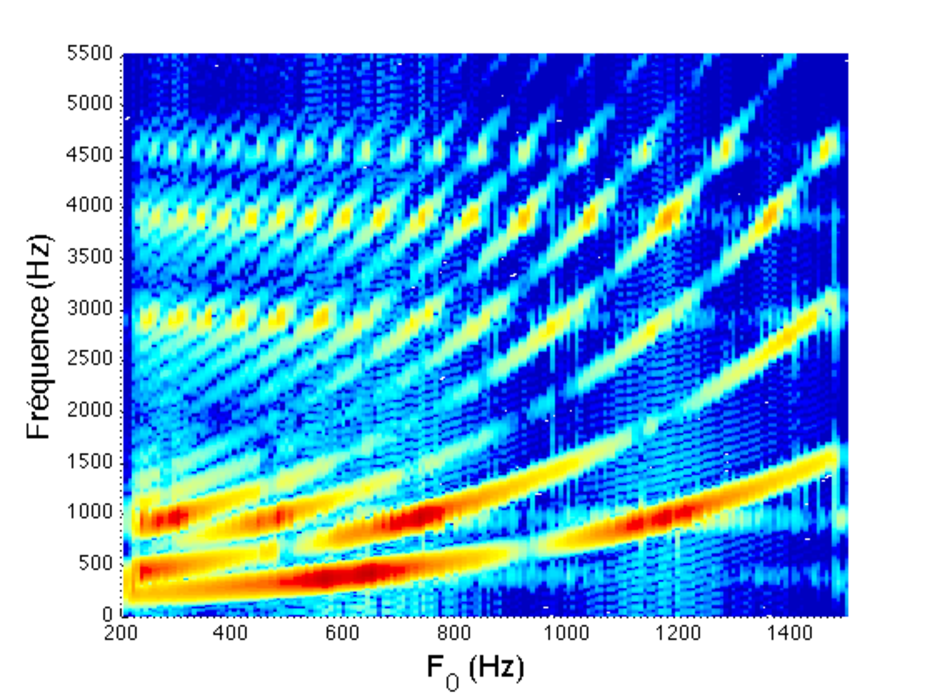
\includegraphics[width=.45\linewidth]{ch2/fig/Fi-F0-dpdce-sans_soprano_u_200-1500Hz_dig13b3.pdf}}
%   \label{Fig:Fi-F0-dpdce_sans}
%   \hspace{0.3cm}
%   \subfloat
% 	[{\it Avec dépendances}]  
%   {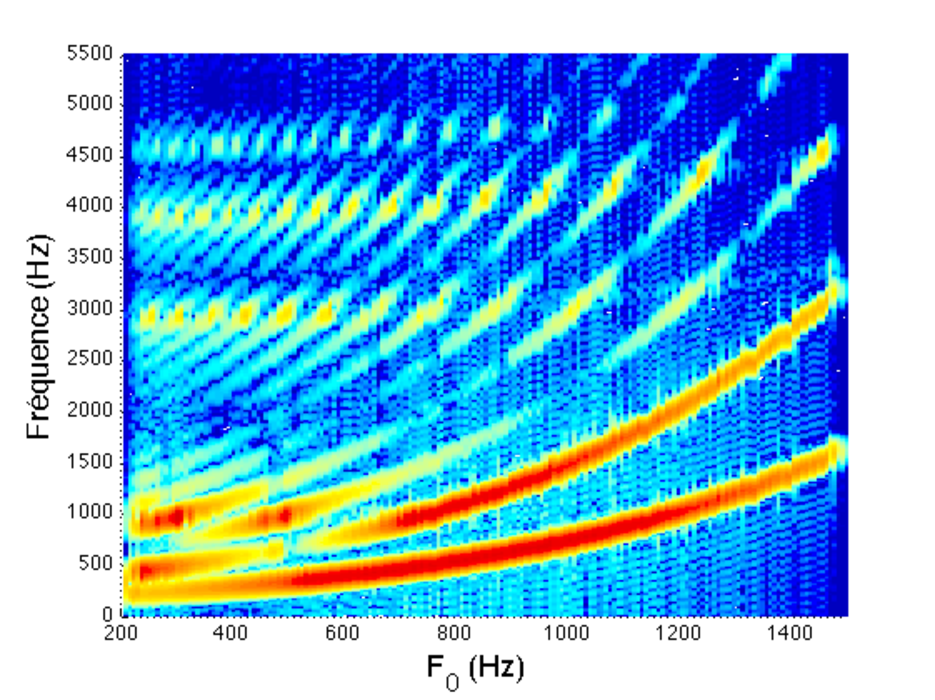
\includegraphics[width=.45\linewidth]{ch2/fig/Fi-F0-dpdce-avec_soprano_u_200-1500Hz_dig13b3.pdf}}
%   \label{Fig:Fi-F0-dpdce_avec}
%     \caption{{\it Spectrogrammes de la voyelle /a/ de synthèse, où $F_0$ augmente avec le temps, (a) sans ou (b) avec les dépendances entre les fréquences centrales des formants et de $F_0$. \textit{Voir fichiers audios~/ vidéos~\ref{fav:fi-f0-dependance}}\\
% }}
%   \label{Fig:Fi-F0-dpdce}
% \end{figure}

% \subsubsection{a) La soufflerie}

% \begin{table}[!h]
% 	\centering
% 	\begin{tabular}{|c|c|c|} 
% 		\hline
% 		& \centering \textbf{Tessiture naturelle moyenne} & \centering \textbf{Tessiture
% dans le synthétiseur} \tabularnewline
% 		\hline
% 		\bf Basse & Mi2-Mi4 & Sol$\sharp$1-Sol4\\
% 		\hline
% 		\bf Ténor & Do3-Si4 & Sol$\sharp$1-Sol4\\
% 		\hline
% 		\bf Alto & Fa3-Mi5 & Sol$\sharp$2-Sol5\\
% 		\hline
% 		\bf Soprano & Si3-Do6 & Sol$\sharp$3-Sol6\\
% 		\hline
% 	\end{tabular}
% 	\caption{\textit{Tessiture des chanteurs naturels et synthétiques (La3=440 Hz). Voir fichiers audios~/ vidéos~\ref{fav:types-voix-1}}}
% 	\label{Tab:tessChant}
% \end{table}

